The magnitude-frequency distributions currently supported by the
\gls{acr:oqe} are the following:

\begin{description}

\item[A discrete incremental magnitude-frequency distribution]
It is the simplest distribution supported. It is defined by the minimum value
of magnitude (representing the mid point of the first bin) and the bin width.
The distribution itself is simply a sequence of floats describing the annual
number of events for different bins. The maximum magnitude admitted by this
magnitude-frequency distribution is just the sum of the minimum magnitude and
the product of the bin width by the number annual rate values. Below we provide an example of the xml that should be incorporated in a
seismic source description in order to define this \gls{acr:mfd}.


\begin{minted}[firstline=1,firstnumber=1,fontsize=\footnotesize,frame=single,bgcolor=lightgray]{xml}
<incrementalMFD minMag="5.05" binWidth="0.1">
    <occurRates>0.15 0.08 0.05 0.03 0.015</occurRates>
</incrementalMFD>
\end{minted}

The magnitude-frequency distribution obtained with the above parameters is
represented in Figure~\ref{fig:evenly_discretized_mfd}.

\begin{figure}[!ht]
\centering
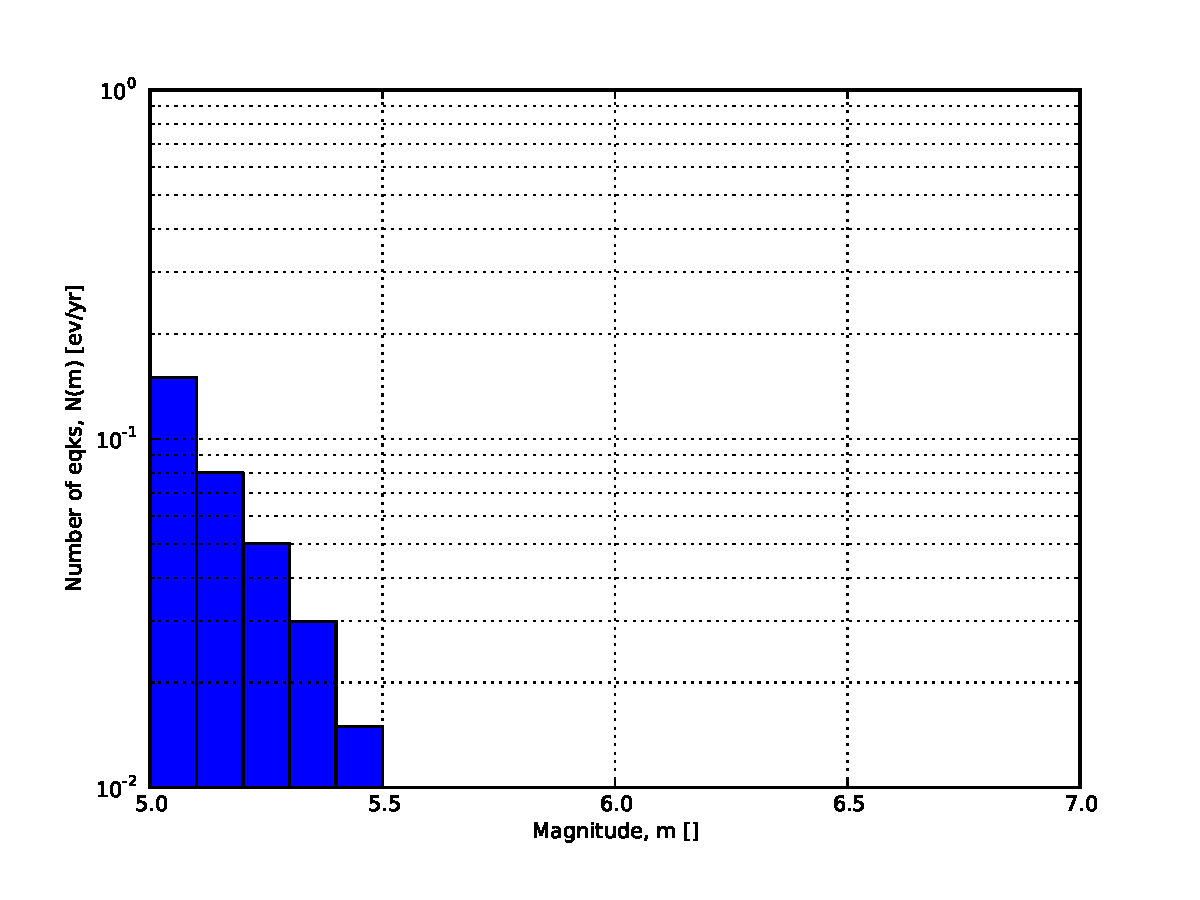
\includegraphics[width=12cm]{figures/hazard/ed_mfd.pdf}
\caption{Example of an incremental magnitude-frequency distribution.}
\label{fig:evenly_discretized_mfd}
\end{figure}

\item[A double truncated Gutenberg-Richter distribution]
This distribution is described by means of a minimum \texttt{minMag} and
maximum magnitude \texttt{maxMag} and by the $a$ and $b$ values of the
Gutenberg-Richter relationship.

The syntax of the xml used to describe this magnitude-frequency distribution
is rather compact as demonstrated in the following example:

\begin{minted}[firstline=1,firstnumber=1,fontsize=\footnotesize,frame=single,bgcolor=lightgray]{xml}
<truncGutenbergRichterMFD aValue="5.0" bValue="1.0" minMag="5.0"
                          maxMag="6.0"/>
\end{minted}

Figure~\ref{fig:dt_gr_mfd} shows the magnitude-frequency distribution
obtained using the parameters of the considered example.

\begin{figure}[!ht]
\centering
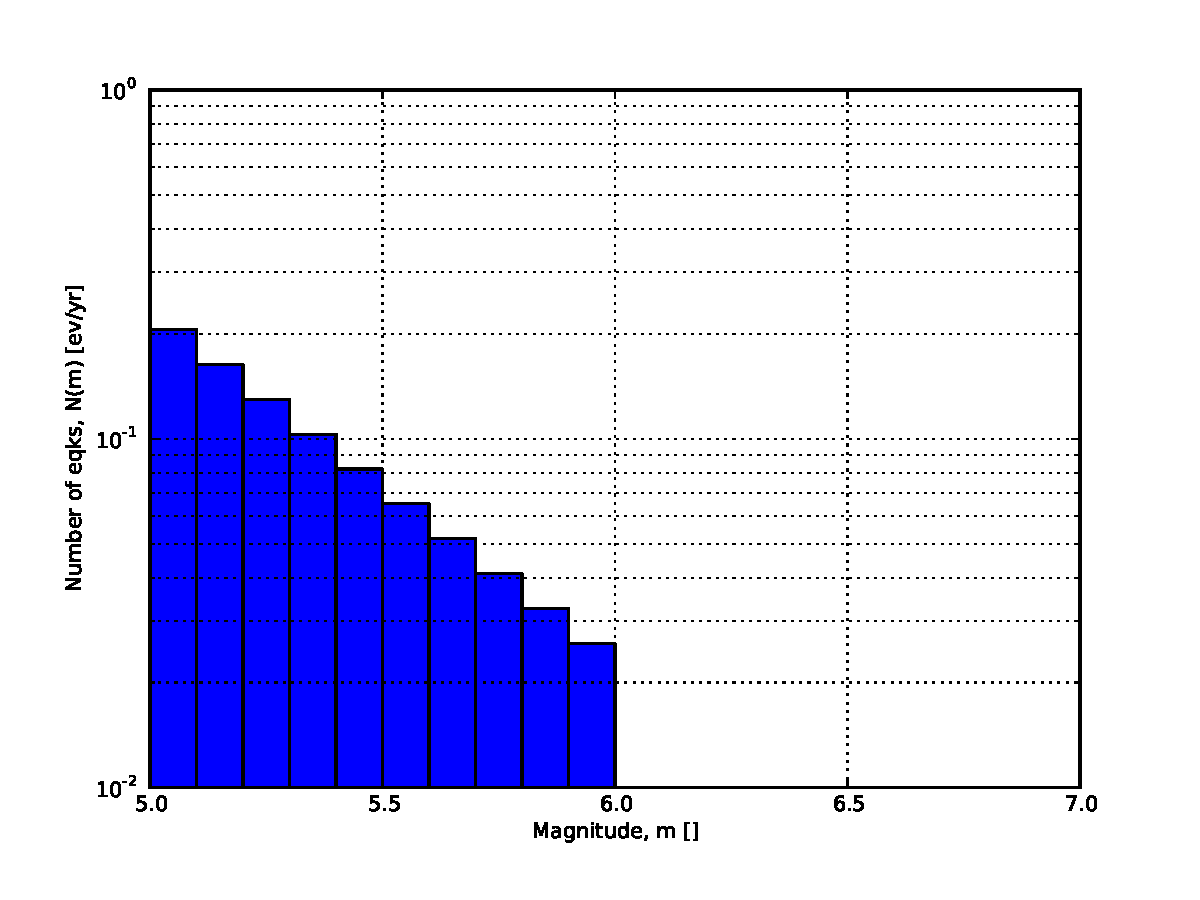
\includegraphics[width=12cm]{figures/hazard/dt_mfd.pdf}
\caption{Example of a double truncated Gutenberg-Richter magnitude-frequency
distribution.}
\label{fig:dt_gr_mfd}
\end{figure}

\item[Hybrid Characteristic earthquake model (\`{a} la \cite{youngs1985})]
The hybrid characteristic earthquake model, presented by \cite{youngs1985},
distributes seismic moment proportionally between a characteristic model (for
larger magnitudes) and an exponential model. The rate of events is dependent
on the magnitude of the characteristic earthquake, the b-value and the total
moment rate of the system (Figure \ref{fig:yc_gr_mfd}). However, the total
moment rate may be defined in one of two ways. If the total moment rate of the
source is known, as may be the case for a fault surface with known area and
slip rate, then the distribution can be defined from the total moment rate (in
N-m) of the source directly. Alternatively, the distribution can be defined
from the rate of earthquakes in the characteristic bin, which may be
preferable if the distribution is determined from observed seismicity
behaviour. The option to define the distribution according to the total moment
rate is input as:


\begin{minted}[firstline=1,firstnumber=1,fontsize=\footnotesize,frame=single,bgcolor=lightgray]{xml}
<YoungsCoppersmithMFD minmag="5.0" bValue="1.0" binWidth="0.1"
                      characteristicMag="7.0" totalMomentRate="1.05E19"/>
\end{minted}


\noindent whereas the option to define the distribution from the rate of
the characteristic events is given as:

\begin{minted}[firstline=1,firstnumber=1,fontsize=\footnotesize,frame=single,bgcolor=lightgray]{xml}
<YoungsCoppersmithMFD minmag="5.0" bValue="1.0" binWidth="0.1"
                      characteristicMag="7.0" characteristicRate="0.005"/>
\end{minted}

Note that in this distribution the width of the magnitude bin must be defined
explicitly in the model.

\begin{figure}[!ht]
\centering
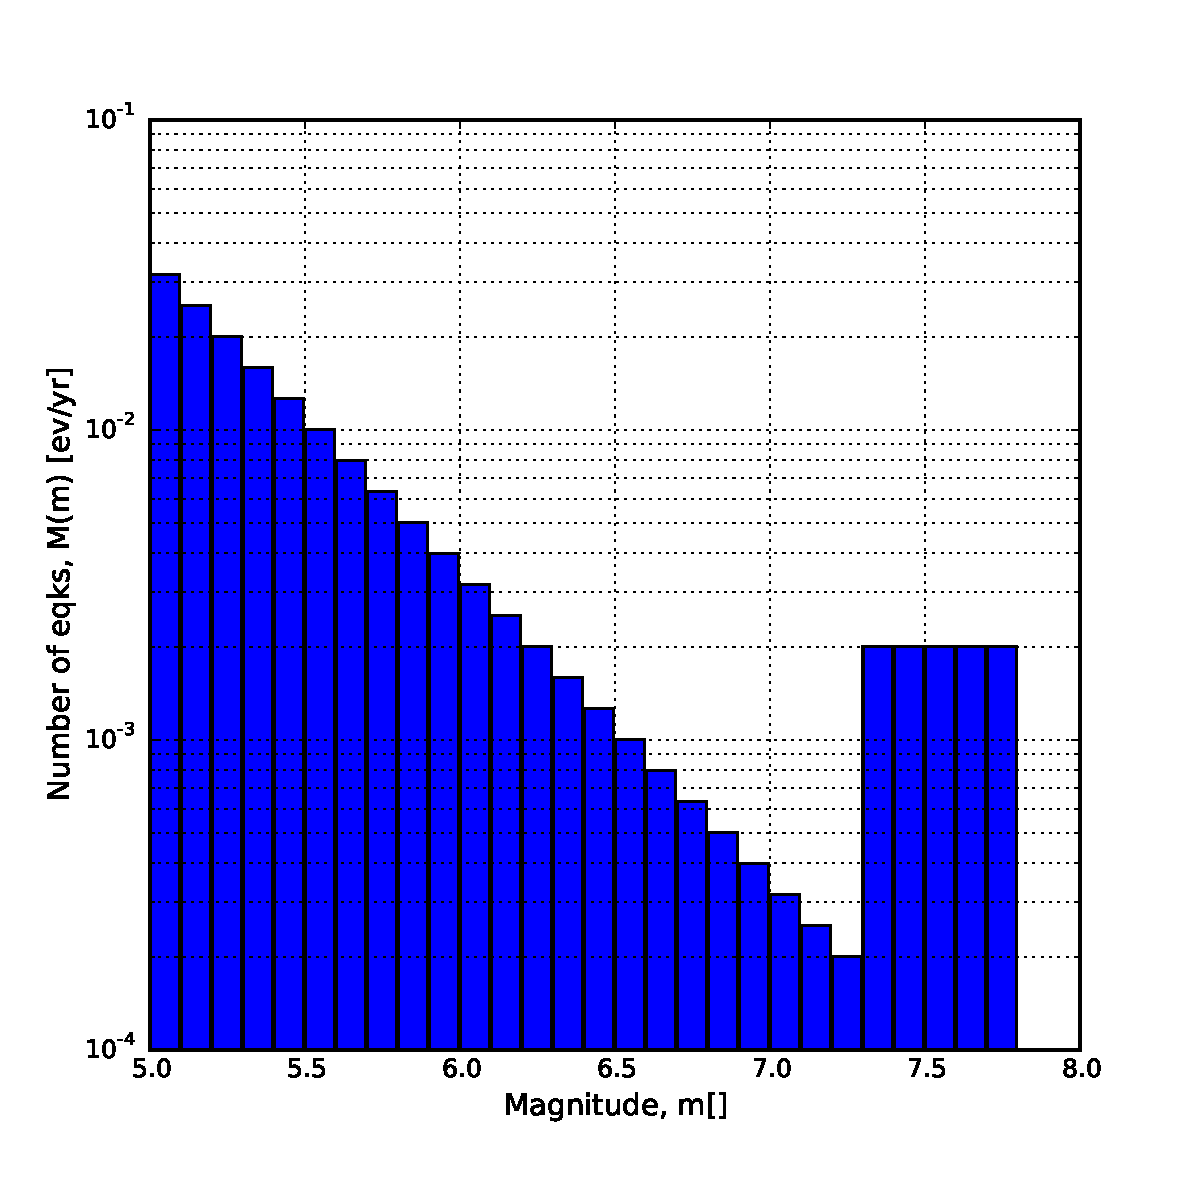
\includegraphics[width=10cm]{figures/hazard/yc_mfd_char_rate.pdf}
\caption{\cite{youngs1985} magnitude-frequency distribution.}
\label{fig:yc_gr_mfd}
\end{figure}

\item[``Arbitrary'' Magnitude Frequency Distribution]
The arbitrary magnitude frequency distribution is another non-parametric form
of MFD, in which the rates are defined explicitly. Here, the magnitude
frequency distribution is defined by a list of magnitudes and their
corresponding rates of occurrence. There is no bin-width as the rates
correspond exactly to the specific magnitude. Unlike the evenly discretised
MFD, there is no requirement that the magnitudes be equally spaced. This
distribution (illustrated in Figure \ref{fig:arb_mfd}) can be input as:

\begin{minted}[firstline=1,firstnumber=1,fontsize=\footnotesize,frame=single,bgcolor=lightgray]{xml}
<arbitraryMFD>
    <occurRates>0.12 0.036 0.067 0.2</occurRates>
    <magnitudes>8.1 8.47 8.68 9.02</magnitude>
</arbitraryMFD>
\end{minted}

\begin{figure}[!ht]
\centering
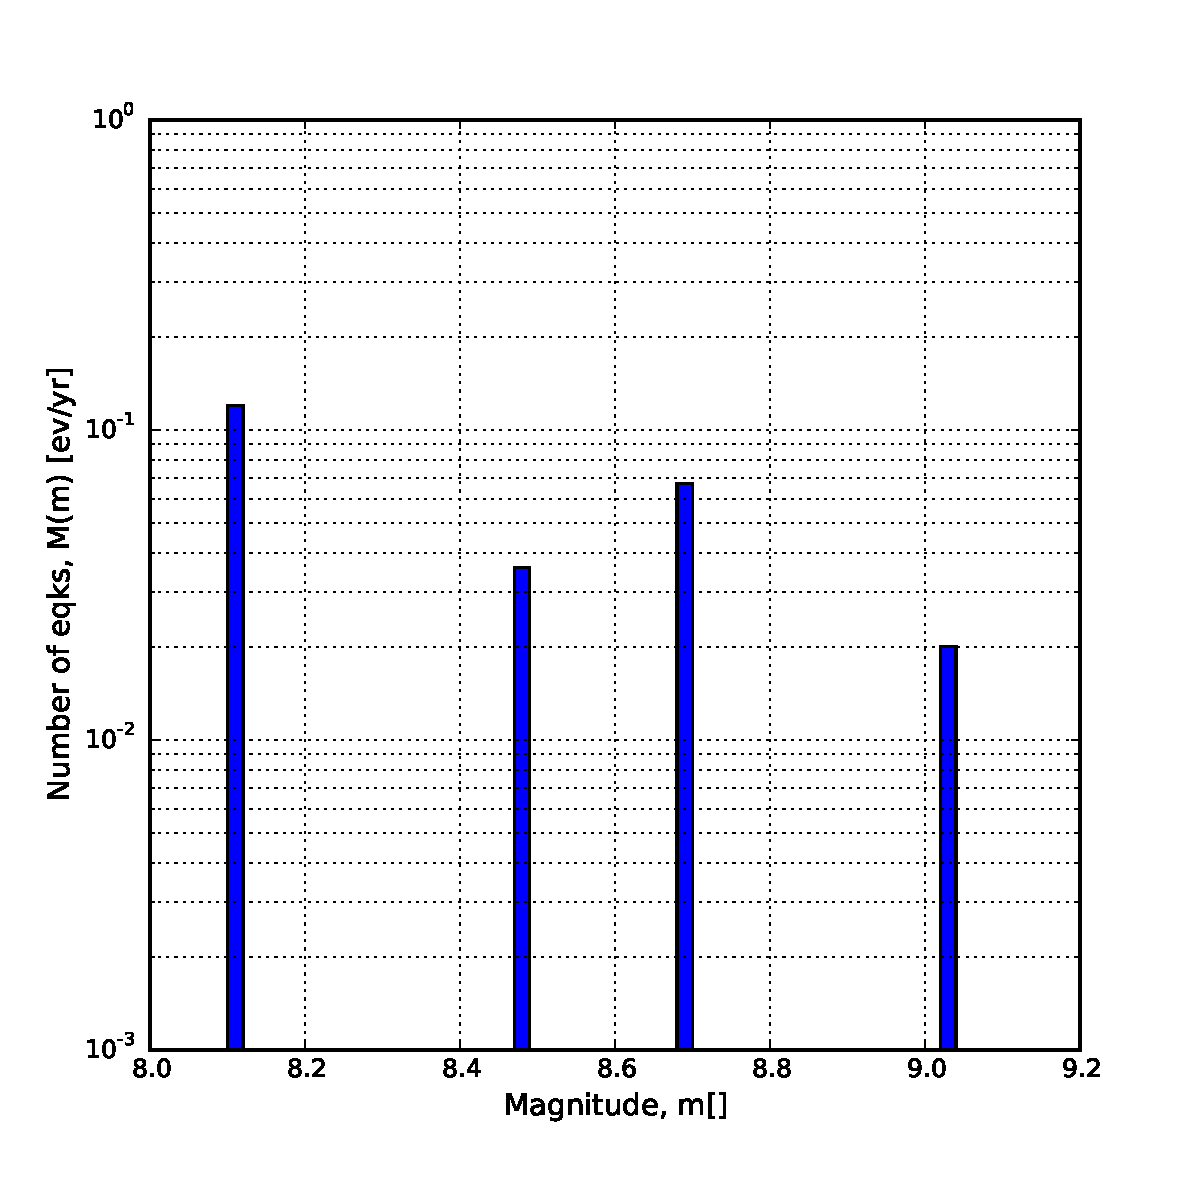
\includegraphics[width=10cm]{figures/hazard/arb_mfd.pdf}
\caption{``Arbitrary'' magnitude-frequency distribution.}
\label{fig:arb_mfd}
\end{figure}

\end{description}